\chapter[Lecture 8]{}\label{lec8}

\section*{Application of representation theory in Quantum Mechanics}

Orthogonal transformation of Coordinate system-
\begin{figure}[H]
\centering
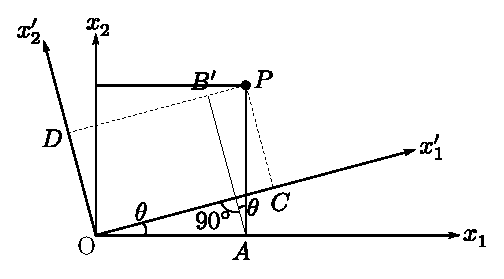
\includegraphics{images/lecture8/fig1.eps}
\end{figure}
\begin{gather*}
x'_{1}=OC=OB+BC=x_{1}\cos \theta+x_{2}\sin\theta B'P=BC\\
a'_{2}=BB'=-AB+AB'=-x_{1}\sin\theta + x_{2}\cos \theta\\
\Rightarrow \ x'_{i}=\sum\limits_{j}a_{ij}x_{j}
\end{gather*}
Keep the axis system fixed, rotate $P$ by $\theta\Rightarrow$ this is equivalent of rotating the axis system by $\theta$ in opposite direction.
$$
\therefore\quad R\in \mathfrak{g}\quad x'=Rx
$$
we define an operator $P_{R}$ such that
$$
\fbox{$P_{R}f(x)=f(R^{-1}x)$}\quad\text{or,}\quad \fbox{$P_{R}f(Rx)=f(x)$}
$$
For two elements $R$, $S\in \mathfrak{g}$
\begin{gather*}
P_{R}f(x)=f(R^{-1}x)=g(x)\\
P_{S}g(x)=g(S^{-1}x)=f(R^{-1}(S^{-1}x))=f((SR)^{-1}x)
\end{gather*}
$a$, $P_{S}P_{R}f(x)=f((SR)^{-1}x)=P_{SR}f(x)\to$ follow group multiplication table $\to$ form a group

\section*{Group of Schr\"odinger Equation}
$$
H=-\dfrac{h^{2}\nabla^{2}}{2m}H\psi=E\psi+v(r)
$$
if $V(r)$ is Coulomb potential $\sim f\left(\dfrac{1}{r}\right)$.

Rotation keep both $\nabla^{2}$ and $v(r)$ invariant
$$
\therefore\quad P_{R}\text{ will commute with } H
$$
Set of all operators that commute with $H$ are called group of Schr\"odinger equation.
$$
\Rightarrow\quad P_{R}H\psi=P_{R}E\psi\Rightarrow H(P_{R}\psi)=E(P_{R}\psi)
$$
if $\psi$ is an eigenstate of $H$, $P_{R}\psi$ is also an eigenstate of $H$. with same eigen value.
$$
\therefore\quad \psi\text{ and } P_{R}\psi\quad\text{are degenerate}
$$
$\therefore$ \ One can find all degenerate states via application of symmetry operation which commute with $H$.
$$
\Rightarrow\quad E_{n}=-\dfrac{E_{0}}{n^{2}}\quad\text{does not depend of } `i', `S'
$$
e.g. if we know $|P_{x}\rangle$ of hydrogen atom. We can find $|P_{y}\rangle$ and $|P_{z}\rangle$ via rotation $\to$ {\bf Normal degeneracy}.
\begin{itemize}
\item In hydrogen atom energy depends on Principal Quantum No. only.

$\therefore$ $RS\rangle$ and $RP\rangle$ are degenerate, but they cannot be produced by symmetry operations $\to$ wave function form is different $\to$ {\bf Accidental Degeneracy}
\end{itemize}

\eject

\noindent
{\bf Speculation}
\begin{itemize}
\item[(i)] There might be some hidden symmetry between them that make them degenerate.

\item[(ii)] Fock proposed that for hydrogen atom one might consider four dimensional rotation symmetry of the `$H$' in momentum space.
\end{itemize}

\noindent
{\bf Representations:} Let us assume $H\psi_{n}=E_{n}\psi_{n}$ and $E_{n}$ in $l_{n}$ fold degenerate {\bf excluding accidental degenerate}
\begin{itemize}
\item $\therefore$ \ we have $l_{n}$ orthonormal eigen functions.

\item They form $l_{n}$ dimensional vector space which is a subspace of the entire Hilbert space.

\item Symmetry/transformation operators can be expressed in terms of matrices $\Gamma$ such that
$$
P_{R}\psi^{(n)}_{\nu}=\sum\limits^{l_{n}}_{k=1}\psi^{(n)}_{k}\Gamma^{(n)}(R)_{k\nu}
$$
$H\psi^{(n)}_{k}=E_{n}\psi^{(n)}_{k}$ for all `$k$'.
\end{itemize}

These representations are {\bf irreducible} as there is always an operator in the group which transform each function to another one degenerate to it.

They follow group multiplication rule.
\begin{align*}
P_{SR}\psi_{\nu} &= P_{S}P_{R}\psi_{\nu}=P_{S}\sum\limits_{k}\psi^{(n)}_{k}\Gamma(R)_{k\nu}\\
&=\sum\limits_{k}(P_{S}\psi_{k})\Gamma(R)_{k\nu}=\sum\limits_{k,\lambda}\psi_{\lambda}\Gamma(S)_{xk}\Gamma(R)_{k\nu}\\
&= \sum\limits_{\lambda}\psi_{\lambda}[\Gamma(S)\Gamma(R)]_{\lambda\nu}\Leftarrow \sum\limits_{k}\Gamma(S)_{\lambda k}\Gamma(R)_{k\nu}=[\Gamma(S)\Gamma(R)]_{\lambda\nu}
\end{align*}
Now, $P_{SR}\psi_{\nu}=\sum\limits_{\alpha}\psi_{\alpha}\Gamma(SR)_{\alpha\nu}$
$$
\therefore\quad \Gamma(SR)=\Gamma(S)\cdot \Gamma(R)
$$
$\therefore \ l_{n}$ degenerate wave functions $\psi^{(n)}_{\nu}$ of energy $E_{n}$ form basis functions for an $l_{n}$-dimensional irreducible representation $\Gamma^{(n)}$ of the {\bf group of the Schr\"odinger equation}.

The representation is {\bf unitary} if one has an orthonormal set of basis functions.

\begin{proof}
Let define Hermitian Scalar product - $(\psi,\phi)=\int\psi^{*}\phi d\tau$
\begin{align*}
\therefore\quad \delta_{k\nu} &= (\psi_{k},\psi_{\nu})=(P_{R}\psi_{k},P_{R}\psi_{\nu})\\
&\quad\text{integral is carried out in rotated coordinate system.}\\
&= \left(\sum\limits_{\lambda}\psi_{\lambda}\Gamma(R)_{\lambda k},\sum\limits_{\mu}\psi_{\mu}\Gamma(R)_{\mu\nu}\right)\\
&= \sum\limits_{\lambda,\mu}(\psi_{\lambda},\psi_{\mu})\Gamma(R)^{*}_{\lambda k}\Gamma(R)_{\mu\nu}\\
&= \sum\limits_{\lambda}\Gamma(R)^{*}_{\lambda k}\Gamma(R)_{\lambda\nu}=\sum\limits_{\lambda}\Gamma(R)^{+}_{k\lambda}\Gamma(R)_{\lambda\nu}\\
&= (\Gamma(R)^{+}\Gamma(R))_{k\nu}
\end{align*}
$\therefore \ \Gamma(R)^{+}\Gamma(R)=E \ \Rightarrow$ matrix representation is unitary.
\end{proof}

\noindent
{\bf Group theory and QM:-}
$\psi_{\nu}$ forms the basis functions in $\Gamma$ representation. Let's assume a different representation $\Gamma'$ with basis $\psi'_{\mu}$ so that 
$$
\psi'_{\mu}=\sum\limits^{l}_{\nu=1}\psi_{\nu}\alpha_{\nu\mu}\quad\text{or}\quad \psi_{k}=\sum\limits^{l}_{\lambda=1}\psi^{1}_{\lambda}d^{-1}_{\lambda k}
$$
\begin{align*}
\therefore\quad P_{R}\psi'_{\mu} &= P_{R}\sum\limits_{\nu}\psi_{\nu}\alpha_{\nu\mu}=\sum\limits_{k,\nu}\psi_{k}\Gamma(R)_{k\nu}\alpha_{\nu\mu}\\
&= \sum\limits_{\lambda,k,\nu}\psi^{1}_{\lambda}\alpha^{-1}_{\lambda k}\Gamma(R)_{k\nu}\alpha_{\nu\mu}=\sum\limits_{\lambda}\psi'_{\lambda}[\alpha^{-1}\Gamma d]_{\lambda\mu}\\
&= \sum\limits_{\lambda}\psi'_{\lambda}\Gamma'(R)_{\lambda\mu}\Rightarrow \fbox{$\Gamma'(R)=\alpha^{-1}\Gamma(R)\alpha$}
\end{align*}
Different choice of basis function merely produces a representation equivalent to the old one.

$\Rightarrow \ \Rightarrow$ Within similarity transformation, there is a unique representation of the Schr\"odinger group for each eigen value of the Hamiltonian.
\begin{itemize}
\item Labels of the representation can be called {\bf good Quantum Number}.

\item A perturbation can lift the degeneracy if and only if, its inclusion reduces the symmetry group [symmetry breaking] and hence changes the irreducible representation.
\end{itemize}

\section*{Abelian Groups}

Each element form a class $\Rightarrow h$ classes and each are {\bf non-degenerate}. $\sum l^{2}_{i}=h$ \ $l_{1}=l_{2}=l_{3}=\ldots l_{h}=1$.

If the symmetry group of Hamiltonian is abelian eigen energies are non-degenerate.

\medskip
\noindent
{\bf Cyclic group:} $A, A^{2},A^{3}\ldots A^{h}=E$

Cyclic group is an abelian group.

Let's assume $\Gamma(A)=r$\quad $\therefore \ \Gamma(A_{n})=r^{n}$
\begin{align*}
 & T(A_{h})=\Gamma(E)\Rightarrow r^{h}=1\\
\therefore\quad &\fbox{$r=e^{2\pi iP/h}$}\quad p=1,2,3\ldots h\\
\therefore\quad &\fbox{$\Gamma^{(P)}(A)=l^{2\pi iP/h}$}
\end{align*}

\medskip
\noindent
{\bf Bloch's Theorem:} Let's assume a periodic potential with period $h$ [linear with periodic boundary condition or a ring]

$A\in \mathfrak{g}$ and $A$ represents displacement by `$a$'.
$$
\therefore\quad P_{A}\psi(x)=\psi(x+a)
$$
$\therefore \ $ All eigen functions of a Hamiltonian having this symmetry must transform according to some representation of a group.

For $p^{\text{th}}$ representation
$$
\psi_{P}(x+a)=P_{A}\psi_{P}(x)=\Gamma^{(p)}(A)\psi_{P}(x)=l^{2\pi iP/h}\psi_{P}(x)
$$
Now, the total length $L=ah$
$$
\therefore\quad \psi_{P}(x+a)=e^{2\pi iPa/L}\psi_{P}(x)=e^{ika}\psi_{P}(x)\quad \fbox{$k=\dfrac{2\pi p}{L}$}
$$
$\therefore$ \ One can easily write $\psi_{P}(x)$ in periodic form.
$$
\fbox{$\psi_{k}(x)=U_{k}(x)e^{ikx}$}
$$
$u_{k}(x)$ is periodic with period $a$.

This is Block Theorem comes rigorously from the consideration of group theory $\to$ no approximation involved

\smallskip

\fbox{$k$ is a good quantum No.} 

\smallskip

Characterizes the eigen function in periodic potential.

\section*{Two dimensional rotation group}

If the axis of rotation is fixed, the rotation group is an abelian group.

e.g., rotation w.r.t. $z$-axis $\to \phi$
$$
\therefore\quad \Gamma(\phi_{1})\Gamma(\phi_{2})=\Gamma(\phi_{1}\phi_{2})
$$
This can be satisfied if $\phi$ comes as exponent 
$$
\therefore\quad \Gamma^{(m)}(\pi \phi)=e^{im\phi}\quad m=0,\pm 1,\pm 2,\ldots
$$
and $T^{(m)}(2\pi)=1=\Gamma^{(m)}(E)$

For a rotation group of a Hamiltonian
$$
\psi_{m}(r,\theta,\phi-\phi_{0})=P_{\phi_{0}}\psi_{m}(r,\theta,\phi)=\Gamma^{(m)}(\phi_{0})\psi_{m}(r,\theta,\phi)=e^{-im\phi_{0}}\psi_{m}(r,\theta,\phi)
$$
$\phi$ depends only through $e^{im\phi}$.

$\therefore \ \psi_{m}$ can be reduced to
$$
\fbox{$\psi_{m}(r,\theta,\phi)=(r,\theta)e^{im\phi}$}
$$
$\Rightarrow$ Angular momentum along an axis is conserved and hence `$m$' is a good quantum no.

\section*{Basis functions for irreducible representations}

Representations of dimensionality greater than $1$ arises from the presence of non-commuting elements.
\begin{itemize}
\item[$\to$] We need two indices (i) row index and (ii) representation index (irreducible)

e.g., $\phi^{(j) \leftarrow \text{representation}}_{k\leftarrow \text{row}}$

\item[$\to$] All the other functions in the same representation, $\phi^{(i)}_{\lambda}$ are called {\bf partners} of $\phi^{(i)}_{k}$
\end{itemize}
Now, 
$$
\fbox{$P_{R}\phi^{(j)}_{R}=\sum\limits^{l_{j}}_{\lambda=1}\phi^{(j)}_{\lambda}\Gamma^{(j)}(R)_{\lambda k}$}
$$
$l_{i}\to$ dimensionality of the representation.

